
\chapter{CTMQC}
\label{chap:CTMQC}


\section{Exact Factorisation}
CTMQC comes from taking the semi-classical limit of an exact factorisation of the molecular wavefunction into its constituent electronic and nuclear components \cite{abedi_exact_2010}. Where the electronic component is parametrically dependent on the nuclear coordinates, $\textbf{R}$. This is shown below in eq \eqref{eq:exact_fact} where $\chi$ is the nuclear wavefunction and $\Phi$ is the electronic one.
\begin{equation}
 \Psi(\textbf{R}, \textbf{r}, t) = \Phi_{\textbf{R}}(\textbf{r}, t) \chi(\textbf{R}, t)
 \label{eq:exact_fact}
 \end{equation}
In the above equation (and throughout this report) I will denote nuclear coordinates and electronic coordinates $R$ and $r$ respectively. The nuclear and electronic wavefunctions then obey separate, but coupled, time-dependent schr\"odinger equations for spatial and temporal evolution. This representation has proven to be useful in furthering understanding through exact solutions of small toy-model systems (need ref \footnote{see deconstruction paper}). However, in this report I will be focussing on the semi-classical limit of these equations (CTMQC) and give some early results of a combination of this and the AOM method explained previously in section \ref{chap:FOB}.
The equations for the evolution of the electronic and nuclear wavefunctions in the exact factorisation \cite{abedi_exact_2010} are given below:
\begin{align}
  i\hbar \frac{\delta}{\delta t} \Phi_{\textbf{R}}(\textbf{r}, t) &= \left( \hat{H}_{BO} + \hat{U}_{en}\left[ \Phi_{\textbf{R}}, \chi\right] - \epsilon(\textbf{R}, t) \right) \Phi_{\textbf{R}} (\textbf{r}, t)
  \label{eq:electronic_exact}
\\
i\hbar \frac{\delta}{\delta t} \chi (\textbf{R}, t) &= \left( \sum_{\nu = 1}^{N_{n}} \frac{[-i\hbar\nabla_{\nu} + \textbf{A}_{\nu}(\textbf{R}, t)]^2}{2 M_{\nu}} + \epsilon(\textbf{R}, t)\right) \chi (\textbf{R}, t)
  \label{eq:nuclear_exact}
\end{align}
Where $\hat{H}_{BO}$ is the Born-Oppenheimer Hamiltonian, that is $\hat{T}_{e} + \hat{W}_{ee} + \hat{W}_{nn} + \hat{V}_{en}$. Where $\hat{T}_{e}$ is the electronic kinetic energy operator, $\hat{W}_{ee/nn}$ is the electron-electron/nuclei-nuclei interation and $V_{en}$ is the electronic-nuclear potential.
\\\\
The $\hat{U}_{en}$ is an electronic-nuclear coupling operator (ENCO). This is defined as \begin{equation}
  \hat{U}_{en}[\Phi_{\textbf{R}}, \chi] = \sum_{\nu=1}^{N_{nuc}} \frac{1}{M_{\nu}} \left[ \frac{\left[-i \hbar \nabla_{\nu} - \textbf{A}_{\nu}(\textbf{R}, t) \right]^2}{2} + \left( \left. \left. \frac{-i\hbar \nabla_{\nu} \chi}{\chi} + \textbf{A}_{\nu}(\textbf{R, t})\right)\right( -i\hbar\nabla_{\nu} - \textbf{A}_{\nu}(\textbf{R}, t)\right) \right]
  \label{eq:ENCO}
\end{equation}
\\
Where the $\textbf{A}_{\nu}$ is a time-dependent vector potential (TDVP), given by $\left\langle \Phi_{\textbf{R}}(t) \right\vert \left. - i \hbar \nabla_{\nu} \Phi_{\textbf{R}} \right\rangle_{\textbf{r}}$ and $M_{\nu}$ is the mass of nuclei $\nu$.
Finally $\epsilon(\textbf{R}, t)$ is a time-dependent scalar potential energy surface (TDPES), given by $\langle \Phi_{\textbf{R}}(t) \vert \hat{H}_{BO} + \hat{U}_{en}^{coup} - i\hbar \frac{\delta}{\delta t} \vert \Phi_{\textbf{R}}(t) \rangle_{\textbf{r}}$.
\begin{wrapfigure}{r}{0.45 \textwidth}
  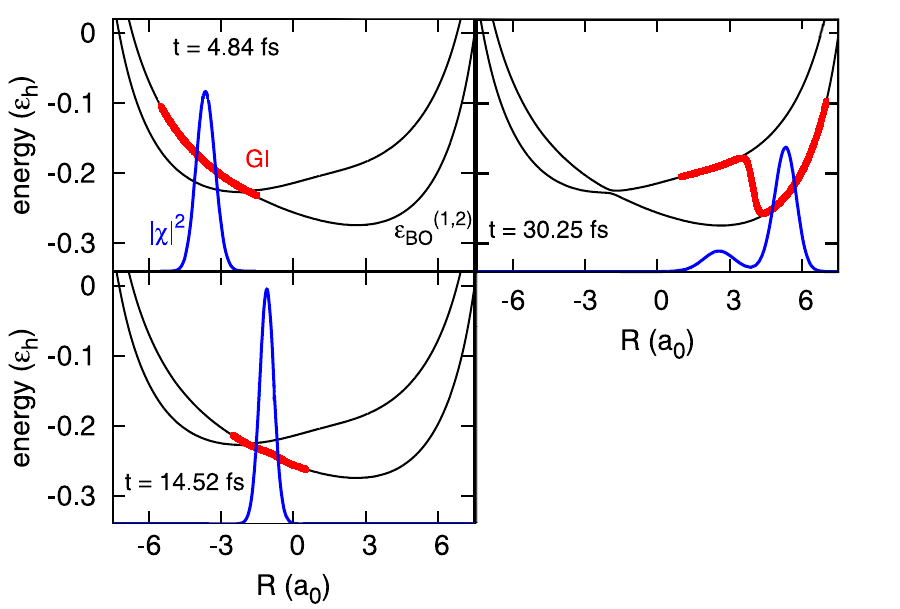
\includegraphics[width=0.7\textwidth]{./img/nuclear_splitting_TDPES.png}
  \caption{A demonstration of how the TDPES can cause the splitting of the nuclear wavepacket in non-adiabatic regions. The red line represents the TDPES and the blue is the nuclear density. Adapted from \cite{agostini_exact_2015} \label{fig:step_TDPES}}
\end{wrapfigure}
\\
The effects of the TDPES, TDVP and the ENCO have been investigated in multiple works \cite{agostini_semiclassical_2015, agostini_exact_2015, agostini_mixed_2013, abedi_dynamical_2013, Min2014Dec}. The TDPES and TDVP are both responsible for the evolution of the system
\cite{agostini_semiclassical_2015}.  The TDPES provides exact classical forces on the nuclei. In fact, an alternative independent-trajectory semi-classical scheme has been investigated using these exact forces \cite{agostini_exact_2015}. This found the TDPES is responsible for the splitting of the nuclear wavepacket in regions of high non-adiabaticity by taking the shape of a step function between the 2 adiabatic potentials. This is demonstrated in figure \ref{fig:step_TDPES}. Finally the electronic-nuclear coupling operator (ENCO) is responsible for the non-adiabatic effects in the system such as electronic nonadiabtic transitions and decoherence \cite{agostini_semiclassical_2015}.
\section{Approximations in CTMQC}
Six approximations have been made in the derivation of CTMQC, these are discussed in detail in Ref. \cite{agostini_quantum-classical_2016}. In the interest of completeness I have summarised them below.
\subsection{Classical Nuclei}
Techniques that include nuclear quantum effects (NQEs); such as multiple spawning \cite{Martnnez*2005Oct}, ring-polymer surface hopping \cite{Shakib2017Jul} and nonadiabatic Bohmian dynamics \cite{Curchod2011Feb, Tavernelli2013Apr} although extremely accurate, cannot be applied to hundreds or thousands of molecules. This is due to their high computational cost. Further, in many systems of interest NQEs are negigible, especially at room temperature. For this reason the classical limit of the nuclear Schr\"odinger equation \eqref{eq:nuclear_exact} is taken when deriving the CTMQC equations.
\subsection{Neglect the ENCO in the TDPES}
The electron-nuclei coupling operator is omitted in the expression for the time-dependent potential energy surface. This is justified as the first term ($\left[-i \hbar \nabla_{\nu} - \textbf{A}_{\nu}(\textbf{R}, t) \right]^2$) contains a second order derivative which is expensive to calculate and has a neglible effect compared to the second term in the ENCO \cite{Scherrer2015Aug}. However, the rest of the ENCO is equal to zero when averaged over $\Phi_{\textbf{R}}(\textbf{r},t)$ so it does not contribute to the TDPES.
\subsection{Derivative of the Adiabatic Coefficients}
The derivative of the adiabatic coefficients appears in the electronic evolution equations. However, we can re-write the derivative of the adiabatic coefficients in terms of their modulus and phase:
\begin{equation}
  \nabla_{\nu} C_{l}^{(I)}(t) = \left[ \underbrace{\frac{\nabla_{\nu} |C_{l}^{(I)}(t)|}{|C_{l}^{(I)}(t)|}}_{(\text{Term 1})} + \underbrace{\frac{i}{\hbar} \nabla_{\nu} \gamma_{l}^{(I)}(t)}_{(\text{Term 2})}\right] C_{l}^{(I)}(t)
\end{equation}
It has been found that the first term is negligible compared to the second \cite{abedi_dynamical_2013, agostini_mixed_2013, agostini_exact_2015} so it doesn't need to be calculated and we can remove it. It was also assumed that the NACVs are localised in space meaning that, after some algebra, the spatial derivative of the adiabatic coefficient can be written as:
\begin{equation}
  \nabla_{\nu} C_{l}^{(I)}(t) = \frac{i}{\hbar} \nabla_{\nu} \gamma_{l}^{(I)}(t) C_{l}^{(I)}(t) = -\frac{i}{\hbar} \int^{t} dt' \nabla_{\nu} \epsilon_{l}^{(I)} C_{l}^{(I)}(t) = -\frac{i}{\hbar} \textbf{f}_{l}^{(I)} C_{l}^{(I)}(t)
  \label{eq:hist_force}
\end{equation}
Where $\epsilon_{l}^{(I)}$ is the energy of the l$^{th}$ adiabatic potential energy surface for trajectory I, $C_{l}^{(I)}$ is the adiabatic expansion coefficient for state l and trajectory I. The $\textbf{f}_{l}^{(I)}$ is the time-integrated adiabatic force.
\subsection{Gaussians as Nuclear Wavepackets}
In order to calculate the quantum momentum -the new term in CTMQC. Knowledge of the nuclear distribution is needed. To this end the nuclear wavepacket is assumed to take the shape of a Gaussian. This is centred on the atomic coordinate with a width $\sigma$. In this work I have used a constant width throughout, with plans to implement dynamic Gaussian width calculations later. However, the nuclei are still propagated classically, the width parameter is only used in the calculation of the quantum momentum.
\subsection{Seperating the Effects of Decoherence and NACVs}
So as to not introduce any population transfer (due to the quantum momentum) when the NACV is zero a fifth approximation has been introduced. Namely the quantum momentum depends on pairs of states -l,k. This enables the seperation of the `competing' effects of the NACV and the Quantum Momentum.
\section{The CTMQC equations}
\subsection{Adiabatic Basis}
The equations for the propagation of the classical nuclei and the expansion coefficients in the CTMQC framework in the adiabatic basis are given below:
\begin{dmath}
  \dot{\textbf{P}}_{\nu}^{(I)} =
  -\overbrace{
     \sum_{k} |C_{k}^{(I)}|^2 \nabla_{\nu}\epsilon_{k}^{(I)}
     - \sum_{k,l} C_{l}^{(I)} C_{k}^{* (I)} \left(\epsilon_{k}^{(I)}  - \epsilon_{l}^{(I)}   \right)
  }^{\text{Ehrenfest}}
  \\
  \underbrace{
    - \sum_{l,k} |C_{l}^{(I)}|^2 \left( \sum_{\nu'=1}^{N_n}    \frac{2}{\hbar M_{\nu'}} \mathcal{Q}_{lk, \nu}^{(I)} \cdot    \textbf{f}_{l, \nu}^{(I)} \right)\left[ |C_{k}^{(I)}|^2    \textbf{f}_{k,\nu}^{(I)} - \textbf{f}_{l,\nu}^{(I)} \right]
  }_{\text{Quantum Momentum}}
    \label{eq:nuc_adiab}
\end{dmath}

\begin{dmath}
  \dot{C}_{l}^{(I)} =
  \overbrace{
    -\frac{i}{\hbar} \epsilon_l^{(I)} C_{l}
    - \sum_k C_k^{(I)} \sum_{\nu=1}^{N_n} \frac{\textbf{P}_{\nu}}{M_{\nu}} \cdot \textbf{d}_{lk, \nu}^{ad, (I)}
  }^{\text{Ehrenfest}} -
  \\
  \underbrace{
    - \sum_{\nu=1}^{N_n}\sum_{k} \frac{\mathcal{Q}_{lk, \nu}^{(I)}}{\hbar M_\nu} \cdot \left[ \textbf{f}_{k,\nu}^{(I)} - \textbf{f}_{l,\nu}^{(I)} \right] |C_{k}^{(I)}|^2 C_{l}^{(I)}
  }_{\text{Quantum Momentum}}
  \label{eq:elec_adiab}
\end{dmath}
Where the $\epsilon_k$ term is the potential energy on the k$^{th}$ potential energy surface. $C_l$ is the adiabatic expansion coefficient corresponding to the l$^{th}$ state. The sum over k and l indicates a sum over all states, the (I) superscript is a replica index and the $\nu$ is an atom index. $M_{\nu}$ is the nuclear mass and $\textbf{d}_{lk, \nu}{^(I)}$ represents the non-adiabatic coupling vector between adiabatic states l and k. The 2 new terms in this scheme not seen in other one are the $\mathcal{Q}_{lk, \nu}^{(I)}$ and the $\textbf{f}_{k, \nu}^{(I)}$. These are the quantum momentum and the history dependent adiabatic force. The history dependent force in defined in equation \eqref{eq:hist_force} this keeps a record of the previous forces in the system. The quantum momentum term couples the trajectories together (making this a coupled-trajectory scheme). Together the history dependent force and quantum momentum are responsible for the decoherence in the `Quantum Momentum' parts of the
above equations \cite{gossel_coupled-trajectory_2018}. Notably, although these equations have been derived from the exact factorisation equations separately from Ehrenfest they do contain exactly the Ehrenfest equations within them (marked `Ehrenfest'). This scheme can therefore be seen as an Ehrenfest scheme with a correction that captures branching of the nuclear wavefunction and decoherence within it.
\\\\
We can also see in equation \eqref{eq:elec_adiab} if we are in a pure adiabatic state i.e. all population on a single adiabatic state, there is no contribution from the quantum momentum part of the equations. In this scenario the evolution equations become simply Ehrenfest equations. For example, if we only have 1 state in the system with non-zero adiabatic population then the term $|C_{k}^{(I)}|^2 C_{l}$ is only non-zero when $l = k$. However, when $l = k$, the term $\left[ \textbf{f}_{k,\nu}^{(I)} - \textbf{f}_{l,\nu}^{(I)} \right]$ is zero as $\textbf{f}_{k,\nu}^{(I)} = \textbf{f}_{l,\nu}^{(I)}$.
Therefore, the quantum momentum term can be seen to only kick in when there is a mixing of adiabatic states. In the adiabatic formulation of these equations it is the adiabatic NACV $\textbf{d}_{lk, \nu}^{ad, (I)}$ that is responsible for the initial mixing of the populations from pure adiabatic states.

\subsection{Diabatic Basis}
The equations above \eqref{eq:nuc_adiab} \& \eqref{eq:elec_adiab} are both in the adiabatic basis. However, to make use of the FOB-formalism detailed in section \ref{chap:FOB} already implemented in the CP2K software package (need ref) these need to be transformed to the orthogonal diabatic basis, $\phi$. After applying the transformation matrix $\mathbb{U}$ and some algebra the equations in the diabatic basis can be written as:
\begin{dmath*}
{ F_{v}^{(I)}(t)} =
\overbrace{ -\sum_{l,k} u_{l}^{(I) *} u_{k}^{(I)} \nabla_{v} H_{lk}^{(I)}}^{\text{Ehrenfest}}
\\
 - \underbrace{2 \sum_{l} |C_{l}^{(I)}|^2 \sum_{n} \left( \sum^{N}_{\nu'} \frac{\mathcal{Q}^{(I)}_{ln,v'}(t)}{\hbar M_{v'}} \cdot \textbf{f}^{(I)}_{l,v'}\right)\left[  |C_{n}^{(I)}|^{2} \textbf{f}^{(I)}_{n,v} - \textbf{f}^{(I)}_{l,v} \right]}_{\text{Quantum Momentum}}
\end{dmath*}

\begin{align*}
\dot{u}_k^{(I)} =
&\overbrace{ - \frac{i}{\hbar}\sum\limits_{l} u_l^{(I)} \left(H_{kl}^{(I)} + i \hbar d_{kl}^{(I)} \right)}^{\text{Ehrenfest}} \\
& + \underbrace{\sum_{s} U_{ks} \sum_{\nu = 1}^{N_n}\sum_{n}^{N_{states}}  \frac{\mathcal{Q}_{sn,\nu}^{(I)}}{\hbar M_\nu}\cdot \left[\vert C_n^{(I)} \vert^2 \mathbf{f}_{n, \nu}^{(I)}- \mathbf{f}^{(I)}_{s, \nu}\right] \sum_{l} U^{*}_{sl} u^{(I)}_{l}}_{\text{Quantum Momentum}}
\end{align*}


{\Large Need to write out the equations in the adiabatic basis and the diabatic basis (can give derivation in the appendix along with conservation of norm). Need to explain the Rlk thing and how to calculate the quantum momentum etc... }
